\documentclass[12pt,a4paper]{article}

% Packages %
\usepackage{titling} % Gives Page Title
\usepackage{setspace} % Gives Ability to use \onehalfspacing and \doublespacing
\usepackage{times} % Time New Roman Font
\usepackage{indentfirst} % Makes the indentation after section
\usepackage{graphicx} % Graphics (Images)
\graphicspath{../images/}

% Bibliography %
\usepackage{natbib}
\usepackage{hyperref}
\bibliographystyle{plain} % Style Here

% Following Are From TablesGenerator.com %
\usepackage[table,xcdraw]{xcolor}
\usepackage{colortbl}

% Title, author, and date %
\title{Interim Report: A Multivariate Approach to Diabetes Risk Assessment}
\author{Brendon Gutierrez \\ \textit{BINF-610: Applied Machine Learning}}
\date{\today}


\begin{document}
	% Generate the title
	\maketitle
	
	% Go to Next Page
	\newpage
	\onehalfspacing
	\section{Background}
	The data for this project is sourced from a Kaggle dataset, which provides information about patients with diabetes. The dataset consists of 768 rows and 9 columns, with the last column serving as the target variable. This dataset can be found \href{https://www.kaggle.com/datasets/akshaydattatraykhare/diabetes-dataset}{here}. The features in the dataset include the number of pregnancies, glucose level, blood pressure, skin thickness, insulin level, body mass index, diabetes pedigree function, and age. Given the limited number of 8 features, the data lacks high dimensionality. Hence, more complex models like neural networks may not be necessary. Nonetheless, some networks will be evaluated to understand how to manage overfitting and underfitting.
	\par 
	Logistic Regression is a fundamental classification algorithm that provides interpretable results, making it a preferred choice for understanding the relationship between features and the target variable. The coding for this section has already commenced, focusing on incorporating various customizable hyperparameter ranges, including different regularization options such as L1, L2, and ElasticNet. To enhance model stability and performance, a Bagging Classifier will be utilized, and hyperparameter tuning will be performed using 5-fold cross-validation.
	\par
	For additional methods, Random Forest and Decision Tree will be employed; while the Random Forest may be more accurate, both approaches are effective given the feature count. Support Vector Machine is considered for its efficacy with non-linear relationships. Despite being potentially excessive, Neural Networks will be tested to gauge their performance and ability to manage overfitting and underfitting. Additionally, Gradient Boosting (XGBoost) will be explored, potentially in combination with techniques like SMOTE and ADASYN to address data imbalance.
	\par
	It is my hypothesis that Random Forest and Decision Trees will produce the highest results due to their ability in low-dimensional datasets. Along with this, further datasets in diabetes will be tested against the models that are trained to see how well they perform in other datasets. Some of them include \href{https://www.kaggle.com/datasets/ehababoelnaga/diabetes-dataset}{this dataset}.
	\par
    \par
    The dataset requires preprocessing to address missing and nonsensical data, particularly where values of 0 are recorded for features like skin thickness, blood pressure, and other variables. Such values are not plausible and need to be handled appropriately to ensure model accuracy. Imputation strategies or excluding these values might be necessary to maintain data integrity.
    \par
    To assess the effectiveness and usefulness of the models, several evaluation metrics will be employed, including accuracy, precision, recall, F1 scores, and ROC AUC. These metrics provide a comprehensive view of model performance, capturing not only overall correctness but also the balance between sensitivity and specificity.
    \par
    Furthermore, model performance will be compared using various resampling techniques such as SMOTE or ADASYN. These techniques are crucial for addressing potential class imbalances within the dataset, ensuring that the models are robust and perform well across different classes. By integrating these methods, the analysis aims to deliver more reliable and generalizable results.
	\par 
	\section{Data Analysis}
	For a comprehensive understanding of the dataset, a series of histograms have been generated. These histograms display the distribution of the data, highlighting the 5\%, median, mean, and 95\% statistics to uncover potential skewness. Additionally, Table 1 provides a concise view of the descriptive statistics. All related code and resources can be accessed \href{https://github.com/brendondgr/Project-BINF610}{here}.
	\begin{figure}[htbp]
		\begin{center}
		\makebox[\textwidth][c]{
		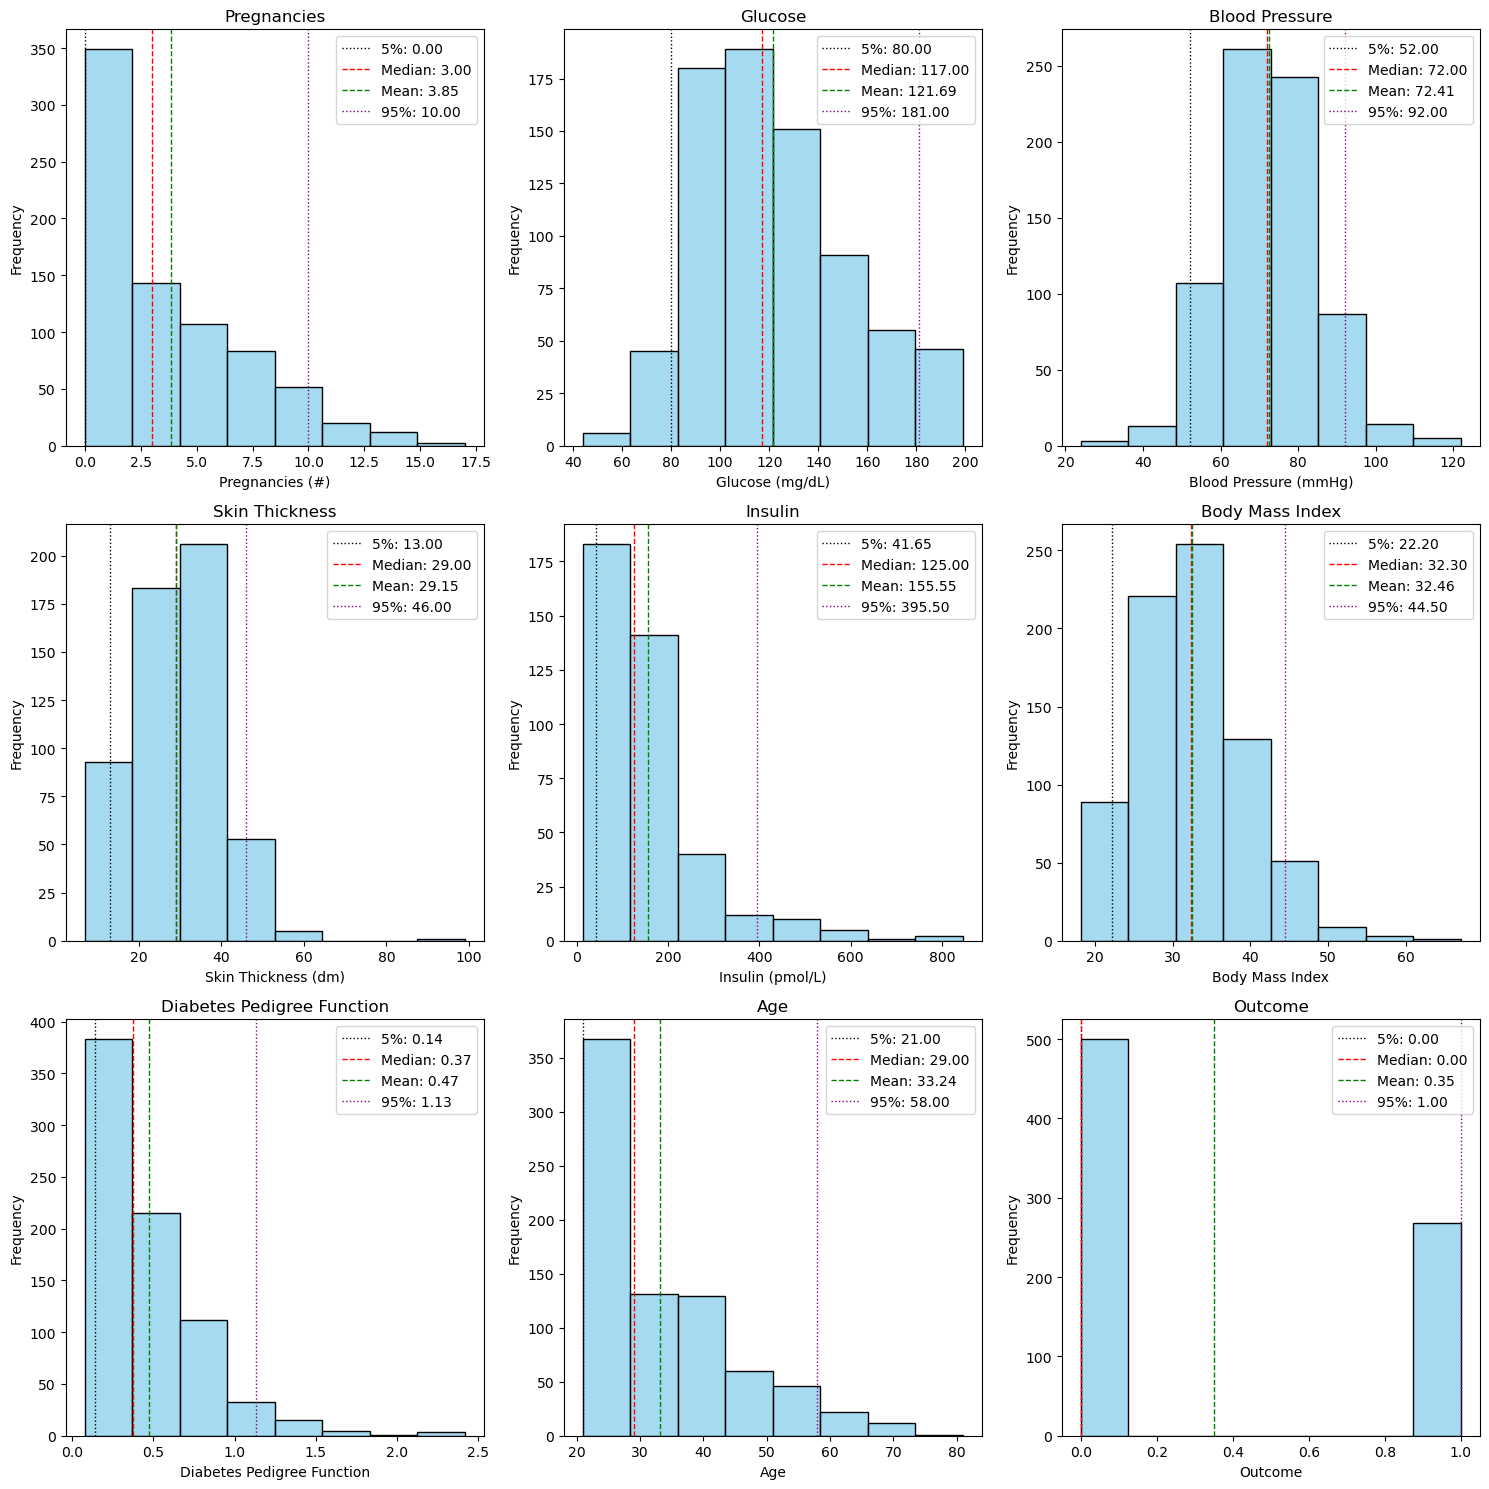
\includegraphics[width=\textwidth]{../images/histograms.png}}
		\caption{Histograms showing the data distribution at various percentiles}
		\label{fig:histograms}
		\end{center}
	\end{figure}
	\begin{table}[]
		\caption{Descriptive Statistics of Diabetes Dataset}
		\label{tab:descriptive_statistics}
		\resizebox{\textwidth}{!} & \textbf{25\%} & \textbf{Median} & \textbf{75\%} & \textbf{95\%} & \textbf{Max} \\
		\textbf{Pregnancies}    & 768            & 3.845         & 3.37         & 0            & 0.0          & 1.0           & 3.0             & 6.0           & 10.0          & 17           \\
		\textbf{Glucose}        & 763            & 121.687       & 30.536       & 44           & 80.0         & 99.0          & 117.0           & 141.0         & 181.0         & 199          \\
		\textbf{Blood Pressure} & 733            & 72.405        & 12.382       & 24           & 52.0         & 64.0          & 72.0            & 80.0          & 92.0          & 122          \\
		\textbf{Skin Thickness} & 541            & 29.153        & 10.477       & 7            & 13.0         & 22.0          & 29.0            & 36.0          & 46.0          & 99           \\
		\textbf{Insulin}        & 394            & 155.548       & 118.776      & 14           & 41.65        & 76.25         & 125.0           & 190.0         & 395.5         & 846          \\
		\textbf{BMI}            & 757            & 32.457        & 6.925        & 18.2         & 22.2         & 27.5          & 32.3            & 36.6          & 44.5          & 67.1         \\
		\textbf{DPF}            & 768            & 0.472         & 0.331        & 0.078        & 0.14         & 0.244         & 0.372           & 0.626         & 1.133         & 2.42         \\
		\textbf{Age}            & 768            & 33.241        & 11.76        & 21           & 21.0         & 24.0          & 29.0            & 41.0          & 58.0          & 81           \\
		\textbf{Outcome}        & 768            & 0.349         & 0.477        & 0            & 0.0          & 0.0           & 0.0             & 1.0           & 1.0           & 1           
		\end{tabular}%
		}
	\end{table}
\end{document}
